\section{Aufbau und Durchführung}
\label{sec:aufbauUndDurchfuehrung}

Der grundlegende Aufbau des Versuchs ist in Abbildung \ref{fig:aufbau} zu sehen.

\begin{figure}
  \centering
  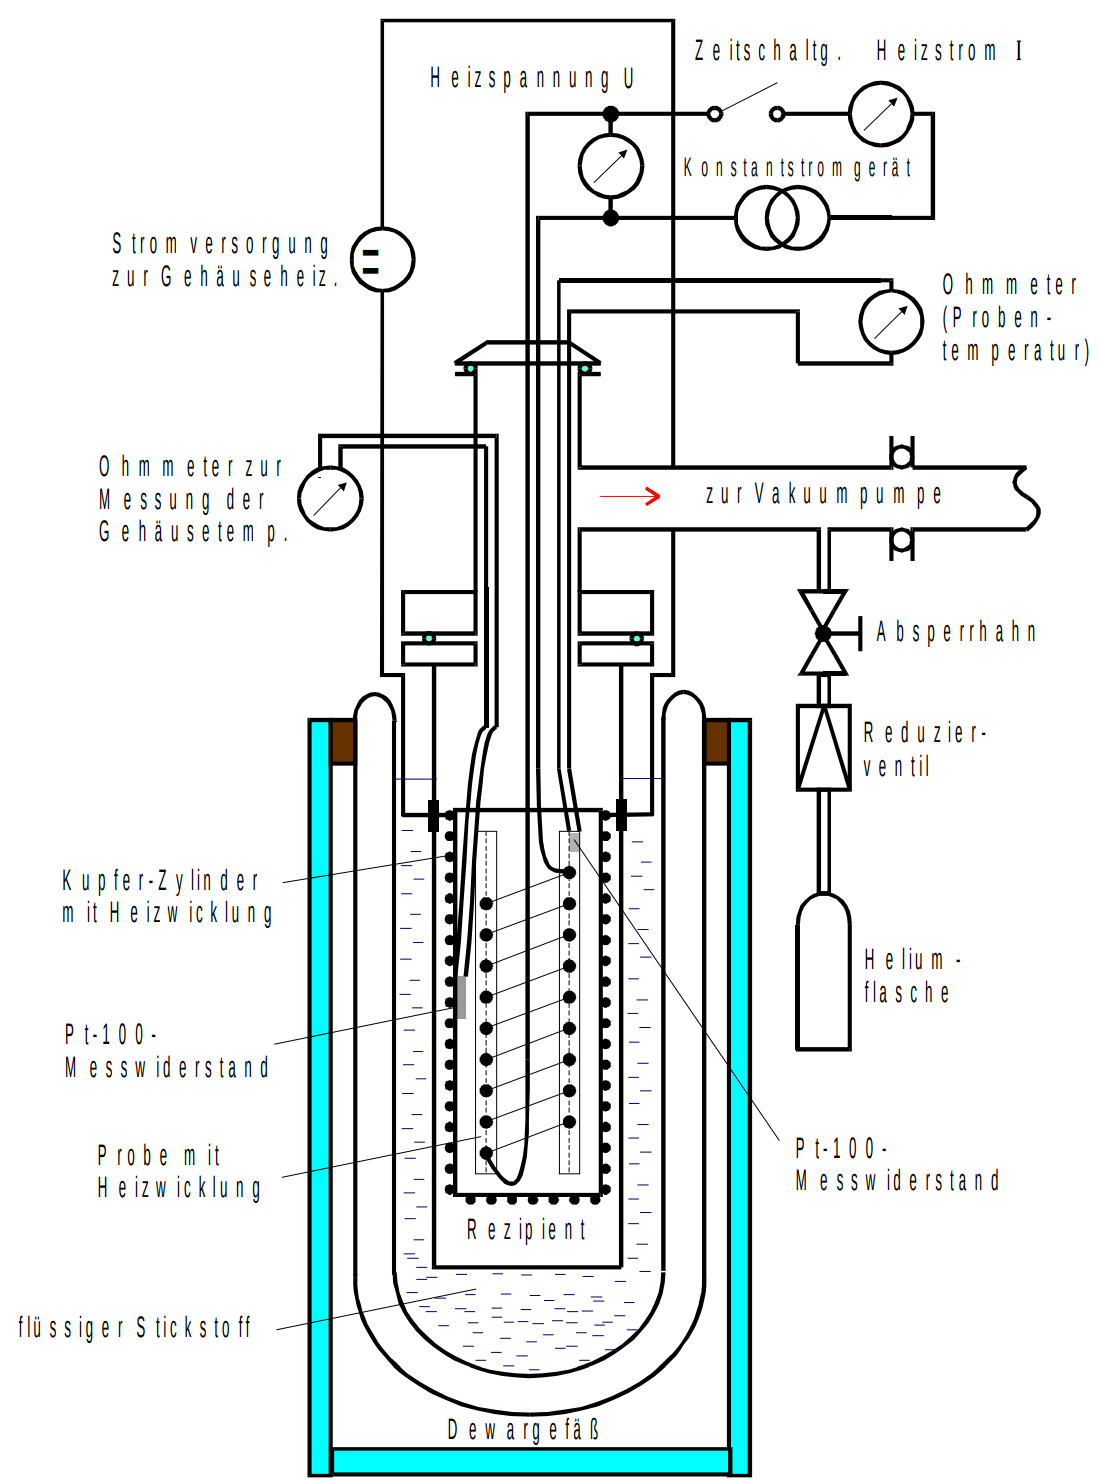
\includegraphics[width=300pt]{data/aufbau.png}
  \caption{Darstellung des Aufbaus mit seinen wesentlichen Komponenten \cite{versuchsanleitung}.}
  \label{fig:aufbau}
\end{figure}

Die Kupferprobe befindet sich in dem Rezipienten und kann über eine Stromversorgung beheizt werden. Um Energieverluste durch Konvektion, Wärmestrahlung und Wärmeleitung gering zu halten, ist der Rezipient während der Messung evakuiert und der die Probe vollständig umgebende Kuper-Zylinder wird möglichst auf der gleichen Temperatur wie die Probe gehalten.\\
Zur Messung der Temperatur und der Probe stehen zwei Pt-100-Widerstände aus Platin zur Verfügung, dessen Widerstand mit digitalen Ohmmetern gemessen wird. Sie sind so kalibriert, dass ihr Widerstand bei $\SI{0}{\celsius}$ gerade $\SI{100}{\ohm}$ beträgt. Da der Widerstand monoton mit der Temperatur anwächst, lässt er sich eindeutig in eine Temperatur umrechnen.

Zunächst wird der Rezipient mithilfe der Vakuumpumpe evakuiert und danach mit Helium gefüllt. Er wird auf ungefähr $\SI{80}{\kelvin}$ abgekühlt. Dies entspricht einem Widerstand von ungefähr $\SI{21.5}{\ohm}$. Die Kühlung erfolgt durch flüssigen Stückstoff, welcher den äußeren Zylinder vollständig umgibt. Nach Erreichen der Zieltemperatur wird die Vakuumpumpe wieder eingeschaltet, um einen möglichst geringen Druck zu erhalten. Die Temperatur des Zylinders wird während der gesamten Messung mit einer Heizstromversorgung kontrolliert und so eingestellt, dass das Widerstandsmessgerät für den Zylinder den gleichen Wert wie das für die Probe zeigt. Da die Apparatur träge reagiert, wird eine Abweichung von bis zu $\SI{1}{\ohm}$ toleriert.

Ab der eingestellten Temperatur von $\SI{80}{\kelvin}$ werden nun in Intervallen von $\SI{150}{\second}$ beide Widerstände, sowie die Spannung und der Strom an der Probe abgelesen. Ab einer Temperatur von circa $\SI{185}{\kelvin}$ und einem Widerstand von ungefähr $\SI{65}{\ohm}$ wird alle $\SI{300}{\second}$ gemessen, bis circa $\SI{25}{\celsius}$ erreicht sind.
